\documentclass[a4paper]{article}
\usepackage{geometry}
 \geometry{
 a4paper,
 total={170mm,257mm},
 left=20mm,
 top=20mm,
 }
\usepackage[english]{babel}
\usepackage[utf8]{inputenc}
\usepackage{amsmath}
\usepackage{graphicx}
\usepackage[dvipsnames]{xcolor}
\definecolor{titleBlue}{RGB}{47, 84, 150}
\usepackage[colorinlistoftodos]{todonotes}
\usepackage{prettyref}
\newrefformat{fig}{Figure~\ref{#1}}
\newrefformat{tab}{Table~\ref{#1}}
\usepackage[colorlinks=true]{hyperref}
\usepackage{float}
\usepackage{fancyhdr}
\pagestyle{fancy}
\fancyhf{}
\lhead{\textcolor{titleBlue}{\textbf{Name:} Viren Chhabria}}
\chead{\textcolor{titleBlue}{\textbf{ID:} 18301780}}
\rhead{\textcolor{titleBlue}{\textbf{Course:} CS7DS1}}
\renewcommand{\headrulewidth}{0pt}

\title{\textbf{\textcolor{titleBlue}{Data Analytics - Final Project}}}

\author{\textcolor{titleBlue}{\textbf{Name:} Viren Chhabria\hspace{2cm}\textbf{ID:} 18301780\hspace{2cm}\textbf{Course:} CS7DS1}}

\date{\textcolor{titleBlue}{\today}}

\begin{document}
\hypersetup{%
    ,urlcolor=blue
    ,citecolor=black
    ,linkcolor=blue
    }
\maketitle

\textcolor{titleBlue}{\section{Introduction}}
\label{sec:introduction}

In this project, the following analysis was performed on the given dataset: \\
\begin{itemize}
    \item Finding the relation between different independent variables with the target label
    \item Visualizing and imputing missing data
    \item Assessing the impact of data imputation on the association between variables
    \item Finding the most important predictors of the target label
\end{itemize}
A heatmap was used for visualizing the correlation between variables and to check the missingness in the data. k-nearest neighbours (kNN) algorithm was used for data imputation. Decision Trees and Random Forest were used to compare the effects of different variables on the target label and to find the variable importance. 

\textcolor{titleBlue}{\section{Methodology}}
\label{sec:methodology}

\textcolor{titleBlue}{\subsection{Dataset}}
\label{sec:dataset}
The dataset consists of 17 attributes and 296 samples. The first attribute was "ID", which was an index to the rows in the dataset. The target label was "Response" which either had class "0" or class "1". X1 - X7 were 7 attributes with continuous values. Y1 - Y7 were 7 categorical attributes, with each class of Y dependent on the respective X attribute having values in a specific range. \\
\prettyref{tab:datasetattrib} shows the attributes in the dataset along with the respective data types. \prettyref{tab:dataset} shows a descriptive overview of the dataset.

\begin{table}[H]
\textbf{\caption{\label{tab:datasetattrib}Dataset Attributes}}
\begin{center}
\begin{tabular}{ |c|c|c| }
 \hline
 \textbf{Attribute} & \textbf{Type} \\
 \hline
 Response & Categorical \\
 \hline
 Group & Categorical \\
 \hline
 X1 - X7 & Continuous \\
 \hline
 Y1 - Y7 & Categorical \\ 
 \hline
\end{tabular}
\end{center}
\end{table}

\begin{table}[H]
\textbf{\caption{\label{tab:dataset}Description of the dataset}}
\begin{figure}[H]
\centering
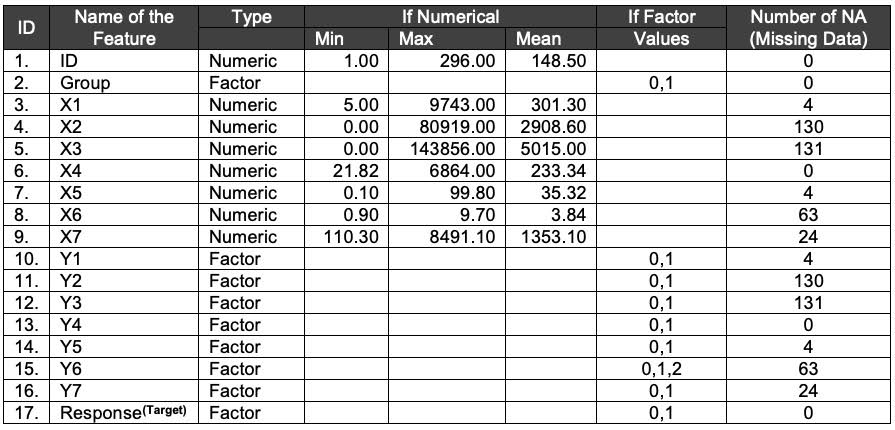
\includegraphics[width=\textwidth]{Dataset.jpg}
\end{figure}
\end{table}

\textcolor{titleBlue}{\subsection{Tools}}
R programming language was used for analyzing the dataset, implementing the algorithms and creating the visualizations(default plot and GGPlot2).

\textcolor{titleBlue}{\subsection{Algorithms}}
\textcolor{titleBlue}{\subsubsection{K-nearest neighbours (kNN)}}
kNN was used in this project for data imputation. It can be used for both, regression and classification. kNN works by finding k existing samples closest to the new given sample, and by majority vote, deciding the value of the given sample.
In R, the "VIM" library was used for the implementation of the kNN algorithm.\\
\textcolor{titleBlue}{\subsubsection{Decision Trees}}
Decision trees are popular and powerful tools used for classification and prediction. They represent rules that can be understood by humans and used in knowledge systems such as a database. Decision tree classifier was used to build a model with the given dataset. 
In R, the "rpart" library was used for the implementation of decision tree classifier.\\
\textcolor{titleBlue}{\subsubsection{Random Forest}}
Random forest is simply an ensemble of decision trees. It uses Bagging and Random Subspace Sampling to build a model. In this project, the random forest was used to determine variable importance and to find the classification error rate trends with respect to the number of trees in the random forest. 
In R, the "randomForest" library was used for the implementation of random forest classifier.
\clearpage
\textcolor{titleBlue}{\subsection{Preprocessing}}

\textcolor{titleBlue}{\subsubsection{Missing Data}}
\label{sec:missingdata}
\prettyref{fig:missingPre} shows the visual representation of the densities of missing values across each attribute in the dataset. Segments represent the sub sections of the dataset. The dataset here was split into 10 segments. "All" indicates the average missing value rate for entire dataset by variables. Overall 15.03\% of data was missing in the dataset.
\begin{figure}[H]
\centering
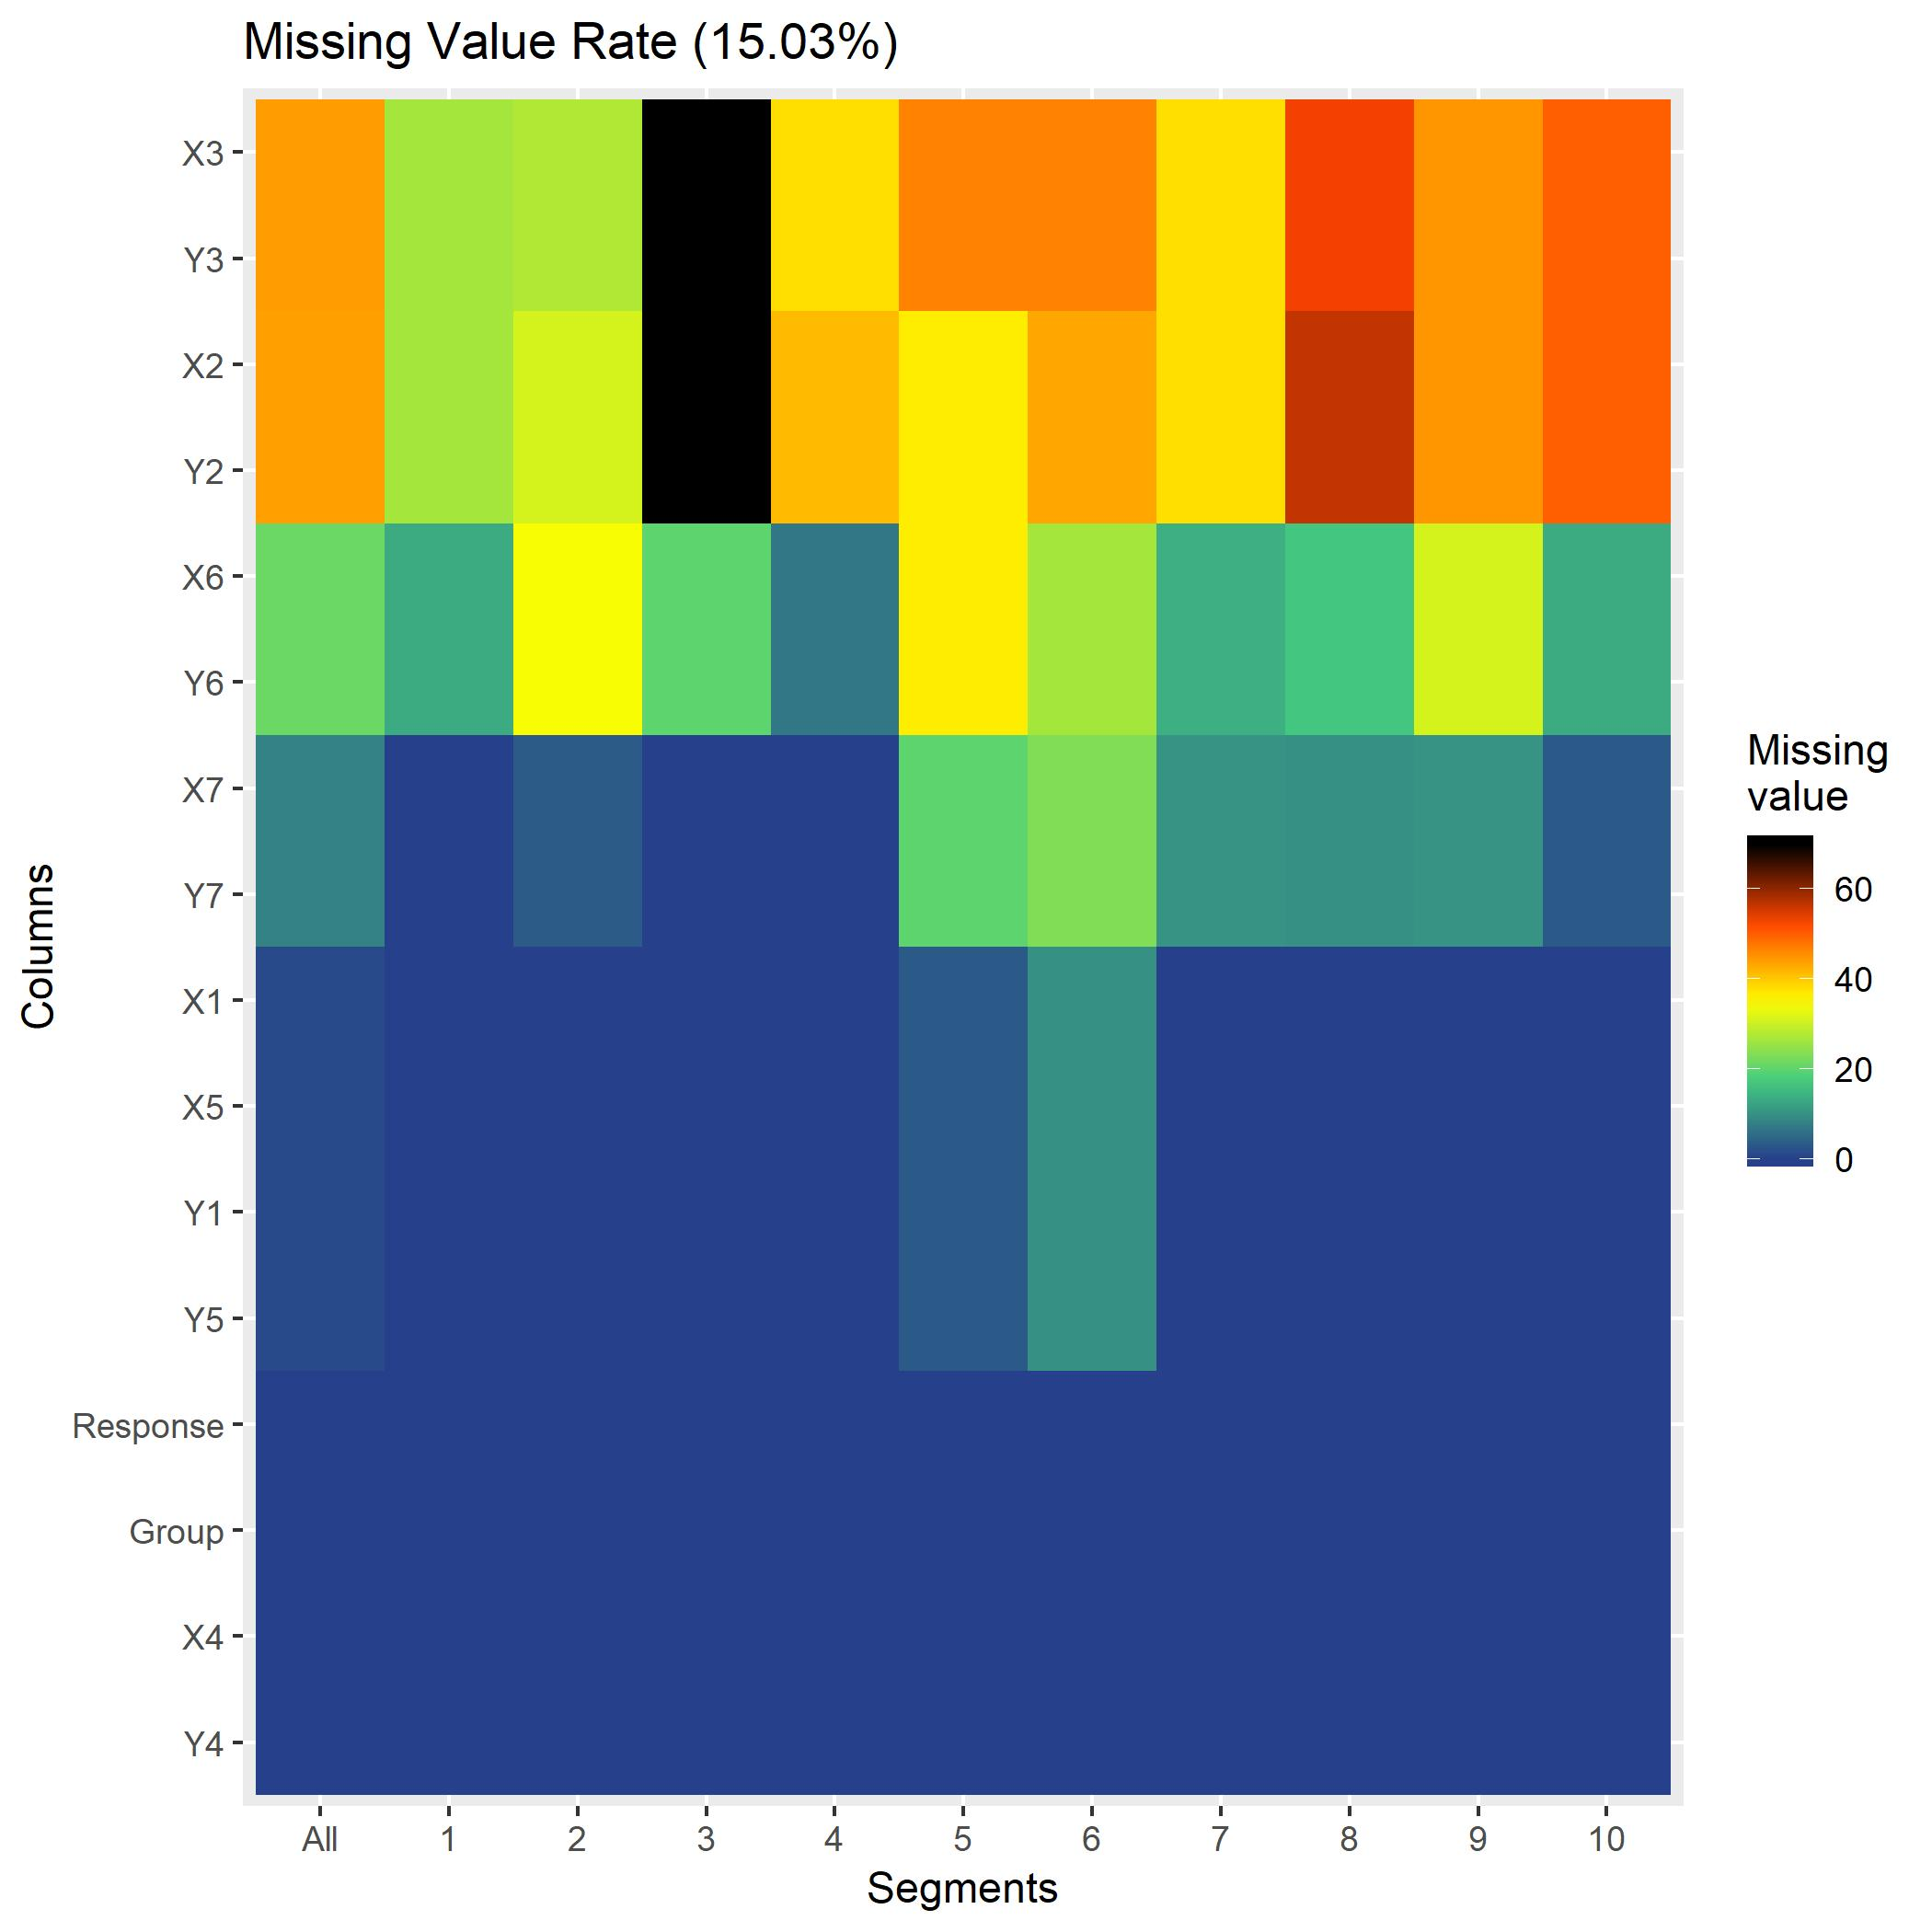
\includegraphics[width=0.7\textwidth,height=0.4\textheight]{HeatmapMissingDataPre.jpg}
\textbf{\caption{\label{fig:missingPre}Missing Data heatmap for all attributes}}
\end{figure}

\textcolor{titleBlue}{\subsubsection{Data Transformation}}
It is known that the Y variables were derived based on the corresponding X variables. For examples, Y1 was derived from X1, Y2 was derived from X2 and so on, though the exact criteria which were used to get the respective Y values from X are not known. Qhile loading the dataset in R, the default datatype of the Y variables in the dataset was taken to be numeric, however, in reality, it was categorical. Therefore data transformation was performed on the Y variables where they were converted from numeric to factors.

\textcolor{titleBlue}{\subsubsection{Feature Removal}}
The first attribute in the dataset, "ID" was an index to the rows in the dataset. It was removed from the dataset, due to its irrelevance to the target label.

\textcolor{titleBlue}{\subsubsection{Data Imputation}}
\label{sec:imp}
The missing data in the given dataset was imputed using K-nearest-neighbours (kNN) algorithm, with the value of k being 5.
\prettyref{fig:preimp} shows the summary of the dataset before imputation, while \prettyref{fig:postimp} shows the summary of the dataset after imputation. Both the figures show that the data imputation didn't alter the mean of the variables too much, except for X2 and X3. \prettyref{fig:missingpostimp} is a heatmap that shows that all the missing data was imputed successfully.\\

\begin{figure}[]
\centering
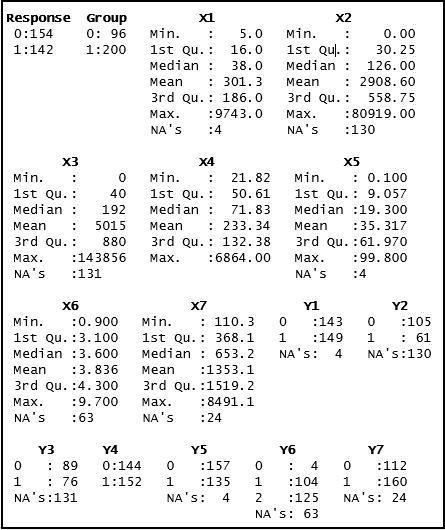
\includegraphics[width=0.5\textwidth, height=0.3\textheight]{DataSummaryPreImp.png}
\textbf{\caption{\label{fig:preimp}Dataset Summary Before Imputation}}
\end{figure}

\begin{figure}[]
\centering
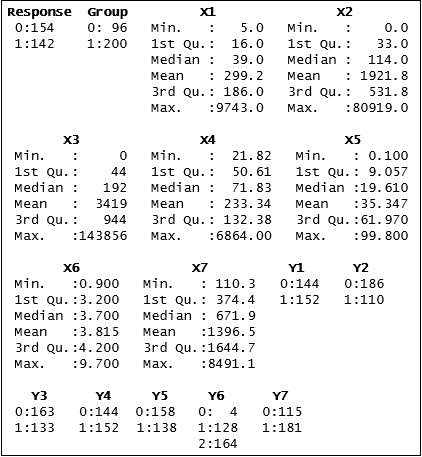
\includegraphics[width=0.5\textwidth, height=0.3\textheight]{DataSummaryPostImp.png}
\textbf{\caption{\label{fig:postimp}Dataset Summary After Imputation}}
\end{figure}

\begin{figure}[H]
\centering
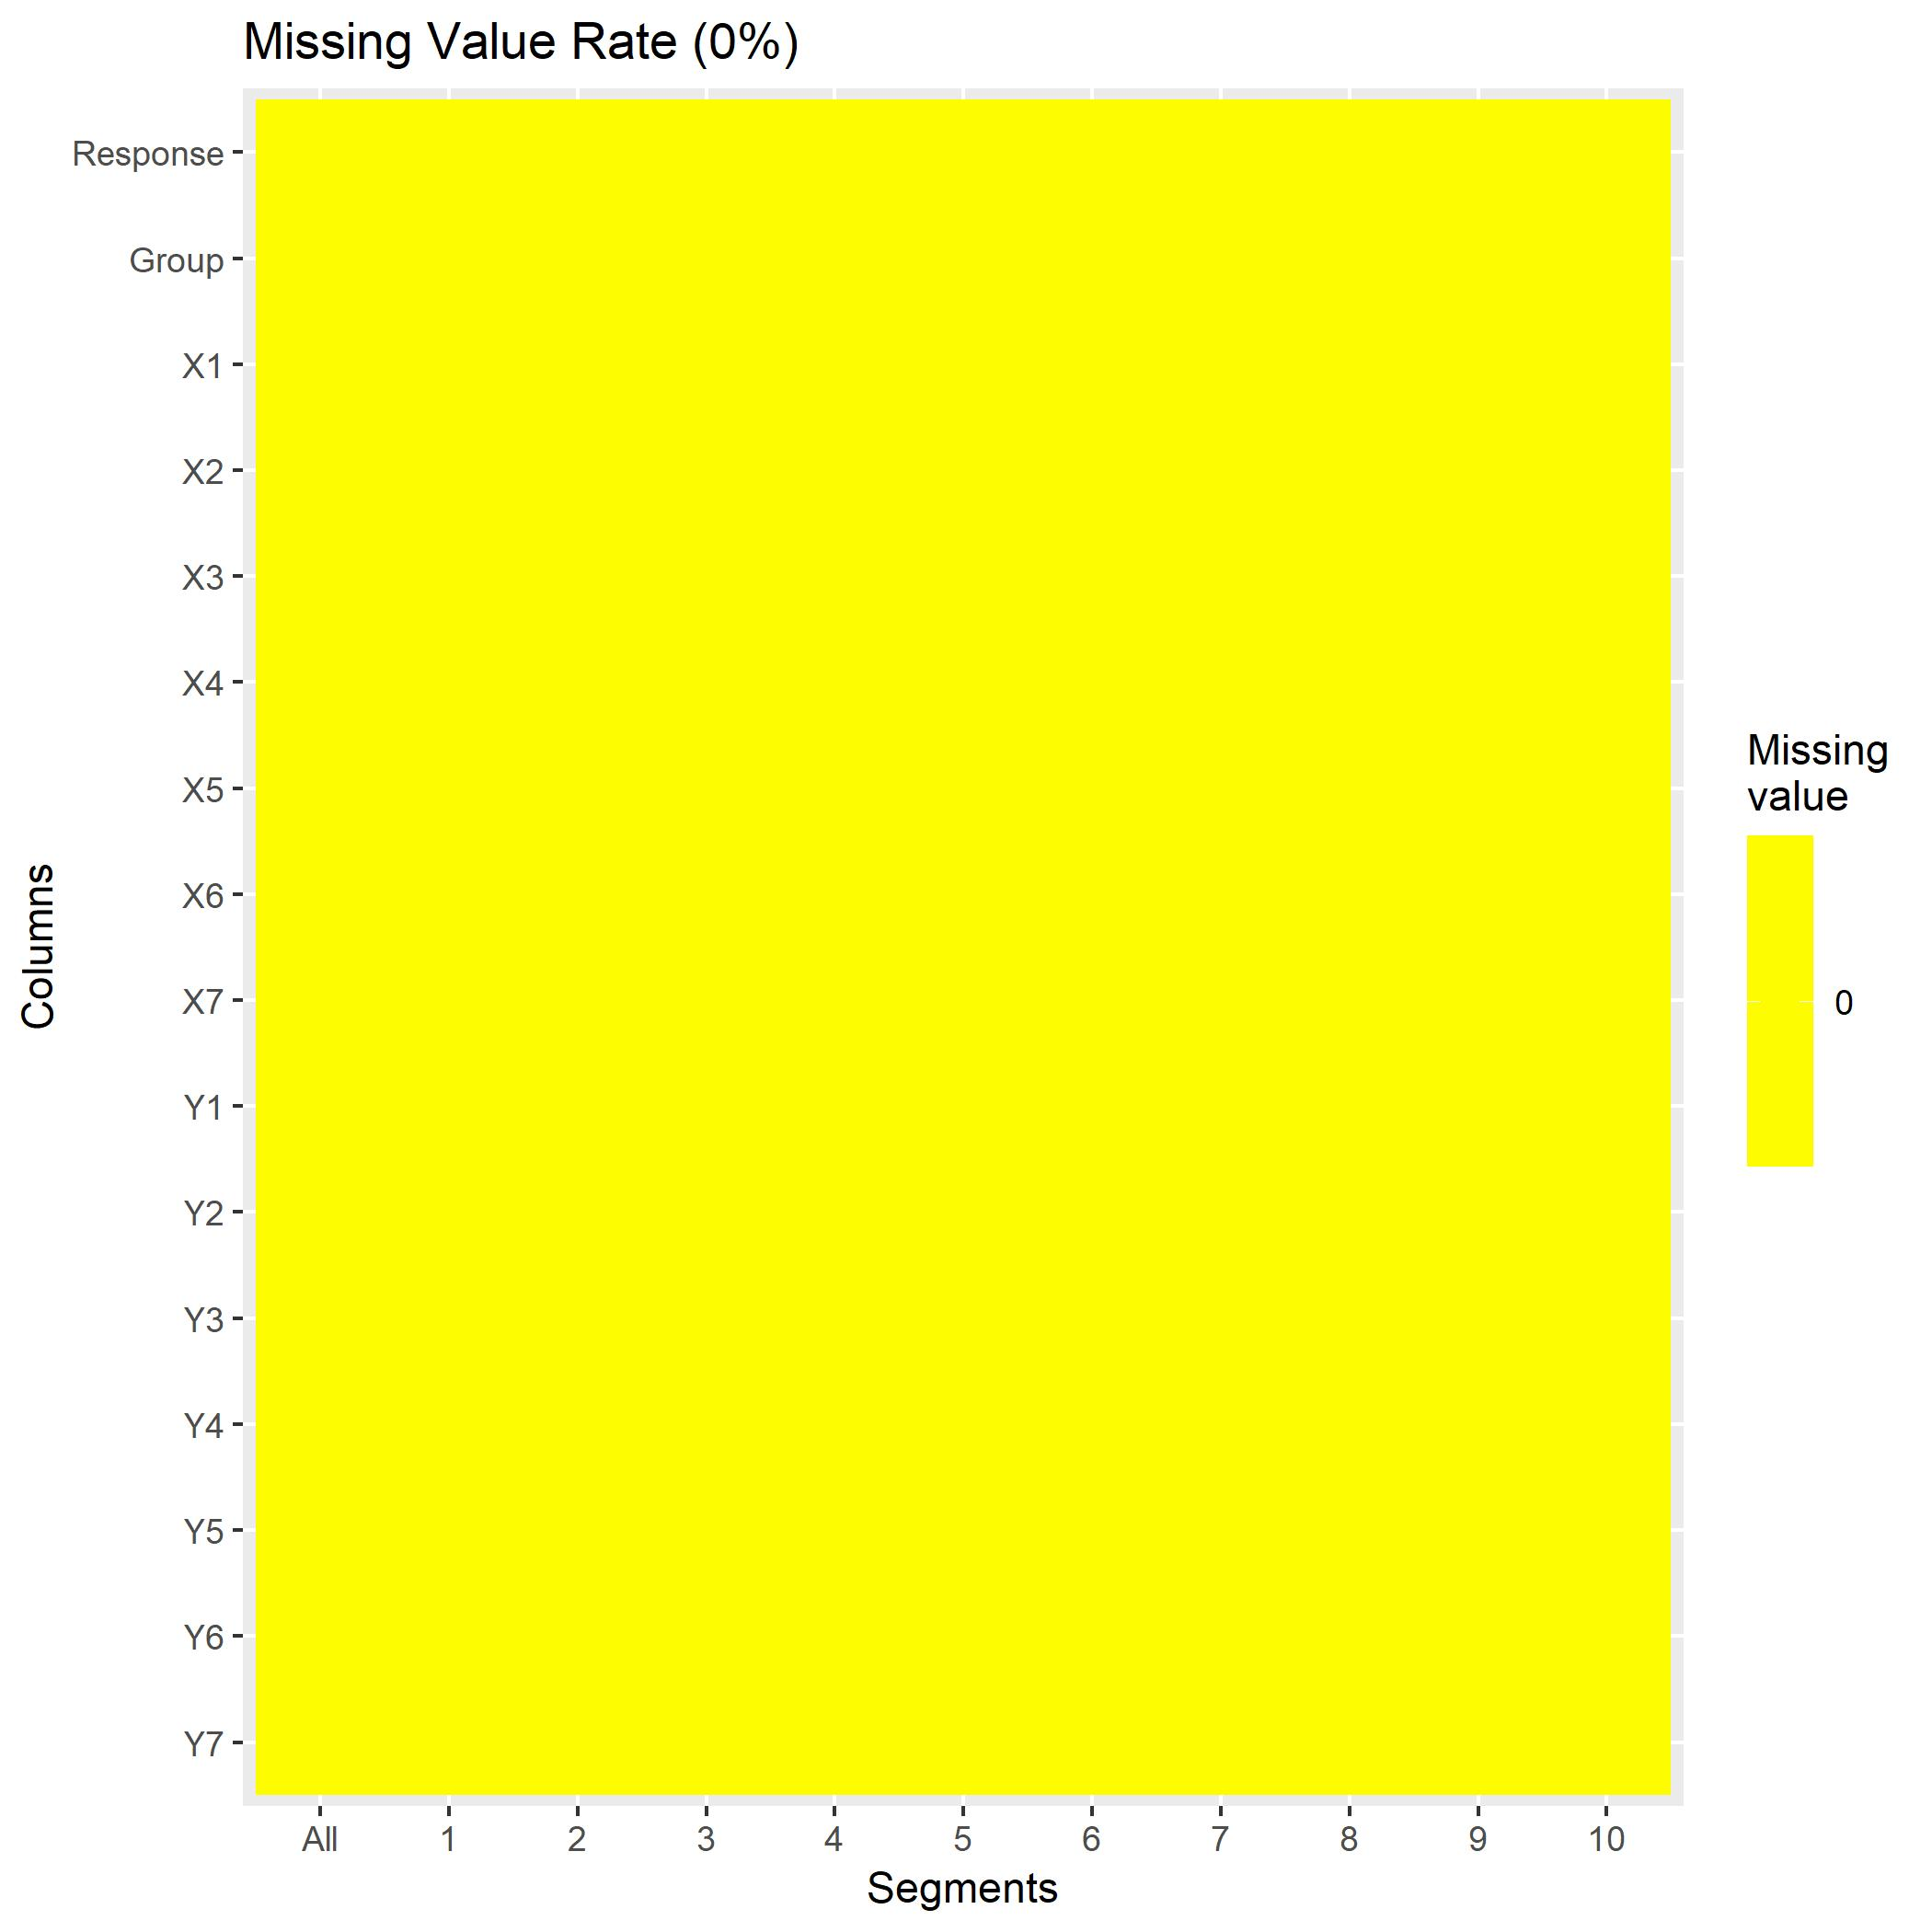
\includegraphics[width=0.7\textwidth,height=0.4\textheight]{HeatmapMissingDataPost.jpg}
\textbf{\caption{\label{fig:missingpostimp}Missing Data heatmap for all attributes after imputation}}
\end{figure}

\textcolor{titleBlue}{\subsection{Evaluation}}
The relationship between the different predictors with the target label "Response" and their importance was assessed by first using different combinations of independent variables to build decision tree's using the original dataset as is, without any data imputation and then repeating the same analysis using the imputed dataset.
The combinations of attributes used were:\\
\begin{enumerate}
    \item All X variables
    \item All X variables plus Group
    \item All Y variables
    \item All Y variables plus Group
    \item All variables
\end{enumerate}

Decision trees can grow extremely large and fit each and every sample in the dataset. This would lead to an overfitted model (high variance). To avoid this scenario, a technique called pruning was applied to control the number of splits in the decision tree by removing sections of the tree that provide little power to classify the instances. All the decision tree's in this project were pruned to the complexity parameter (CP) corresponding to the minimum cross-validation error (xerror). 
\clearpage
\textcolor{titleBlue}{\section{Results and Discussion}}
\label{sec:discussion}
\textcolor{titleBlue}{\subsection{Correlation}}
\label{sec:correlation}
Correlation matrix can be derived for numerical values, to understand the relationship between 2 variables. Heatmap's were created to visualize the relation between the various X values.
\prettyref{fig:correlation} shows the correlation heatmap before data imputation and \prettyref{fig:correlationpost} shows the correlation heatmap after data imputation. There is no visible changes in the correlation between the X variables after data imputation. X2 and X3 are highly correlated in both the cases, hence one of them can be removed while building the model.

\begin{figure}[H]
\centering
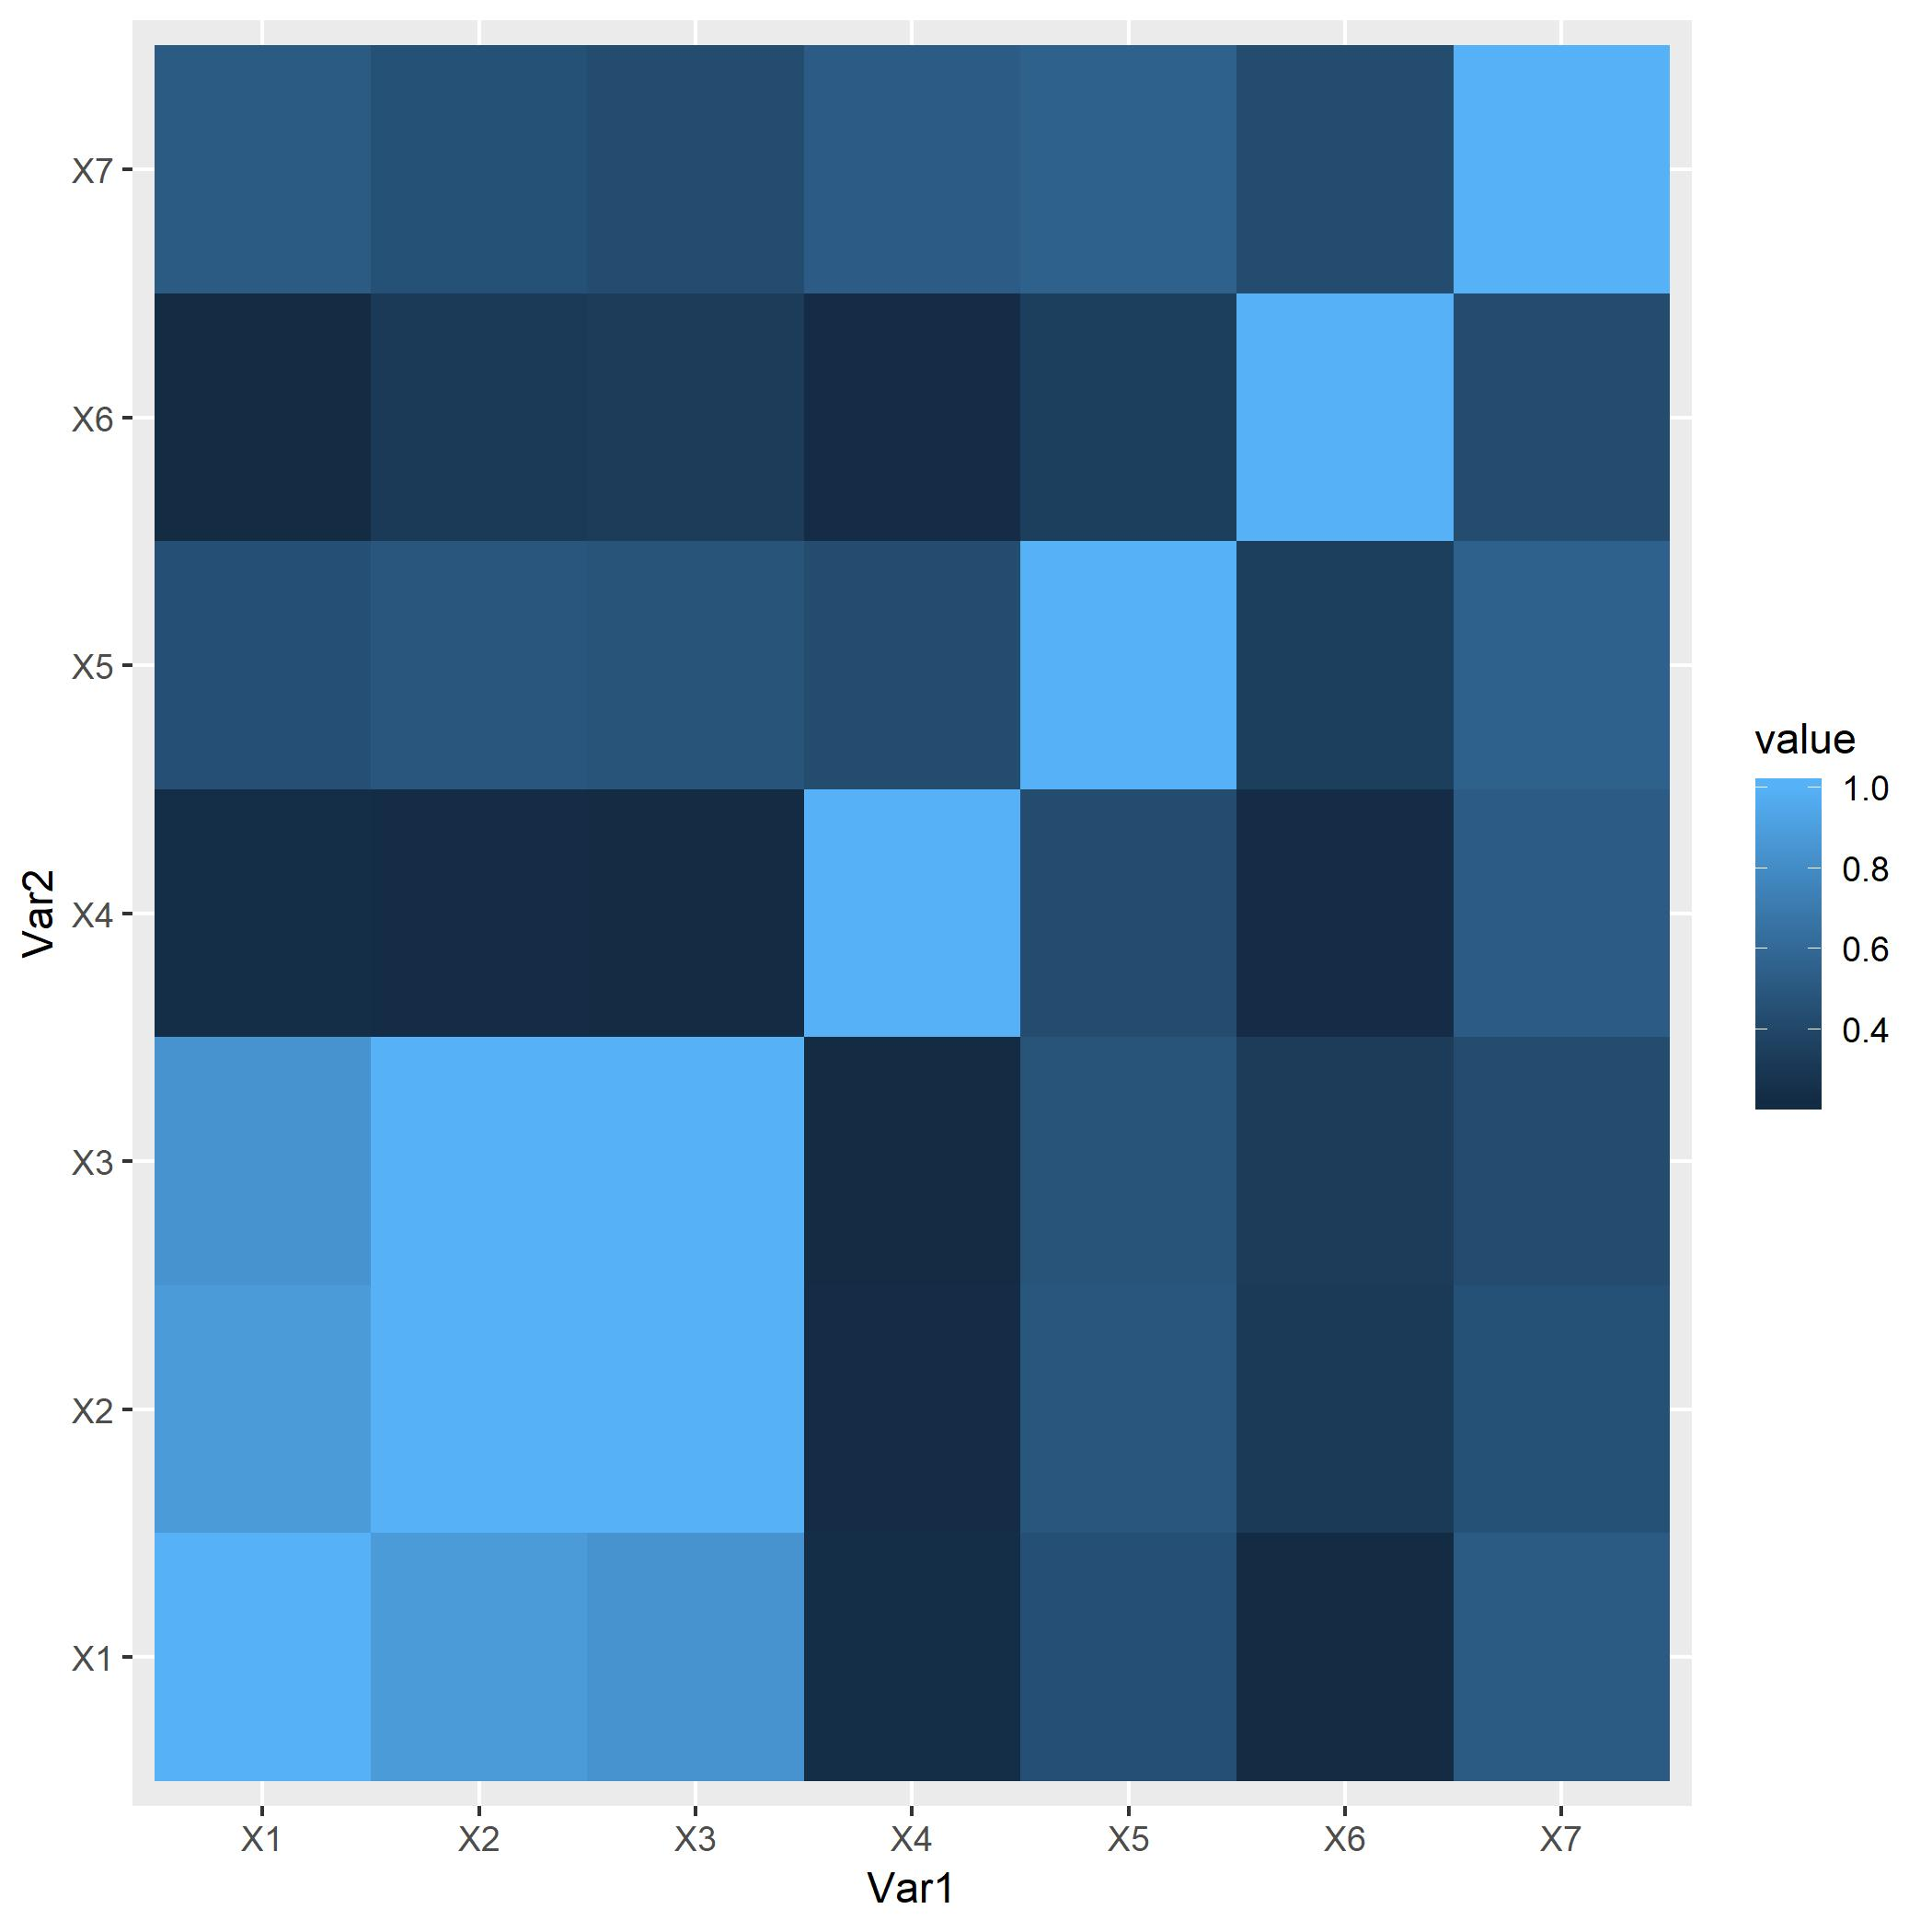
\includegraphics[width=0.55\textwidth,height=0.34\textheight]{CorrelationHeatmapWithMissingData.jpg}
\textbf{\caption{\label{fig:correlation}Coorelation heatmap for X1 - X7 attributes before data imputation}}
\end{figure}

\begin{figure}[H]
\centering
\includegraphics[width=0.55\textwidth,height=0.34\textheight]{{"Correlation Heatmap- with kNN imputed Data"}.jpg}
\textbf{\caption{\label{fig:correlationpost}Coorelation heatmap for X1 - X7 attributes after data imputation}}
\end{figure}

\textcolor{titleBlue}{\subsection{Decision Tree}}
\label{sec:decisiontree}
\begin{enumerate}
    \item \textbf{All X Variables}\\\\
Decision tree with only X variables, before data imputation had only 2 splits, however, post data imputation, 5 splits was found to have the lowest cross validation error. X1 and X4 remained significant splits in both the trees as shown in \prettyref{fig:AllX} and \prettyref{fig:AllXpost}.
\begin{figure}[H]
\centering
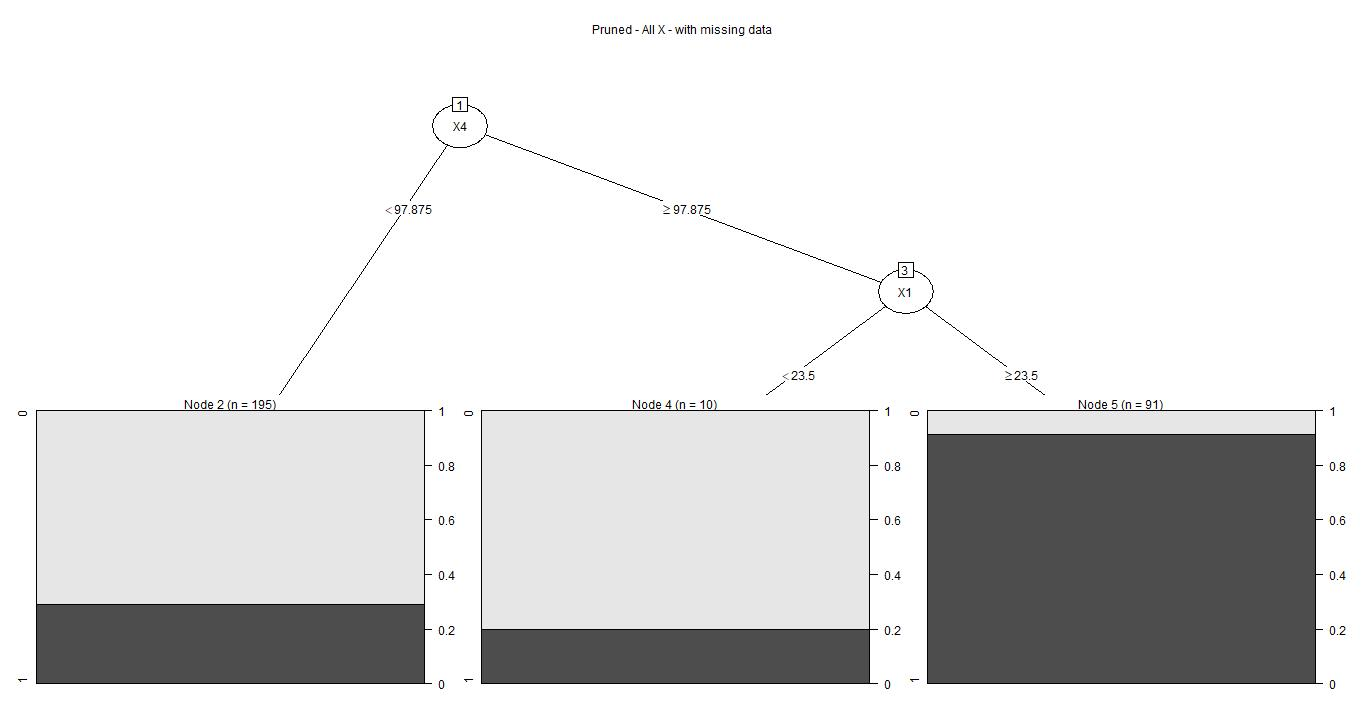
\includegraphics[width=\textwidth, height=8cm]{AllX-withMissingData.jpg}
\textbf{\caption{\label{fig:AllX}Pruned Decision Tree - All X variables as predictors before data imputation}}
\end{figure}

\begin{figure}[H]
\centering
\includegraphics[width=\textwidth, height=8cm]{{"All X - with kNN imputed Data"}.jpg}
\textbf{\caption{\label{fig:AllXpost}Pruned Decision Tree - All X variables as predictors after data imputation}}
\end{figure}

\clearpage

    \item \textbf{All X variables plus Group}\\\\
Considering "Group" along with the X variables had some impact on the decision tree using the dataset with missing values. \prettyref{fig:AllXG} shows that the best number of splits went up from 2 in the previous case to 9 in this case (overfitted model) for the decision tree before data imputation. After data imputation the best split decision tree remained the same as the previous case as shown in \prettyref{fig:AllXGpost}. "Group" variable was not considered for a split in either tree, and X4 remained the root node in both cases.
\begin{figure}[H]
\centering
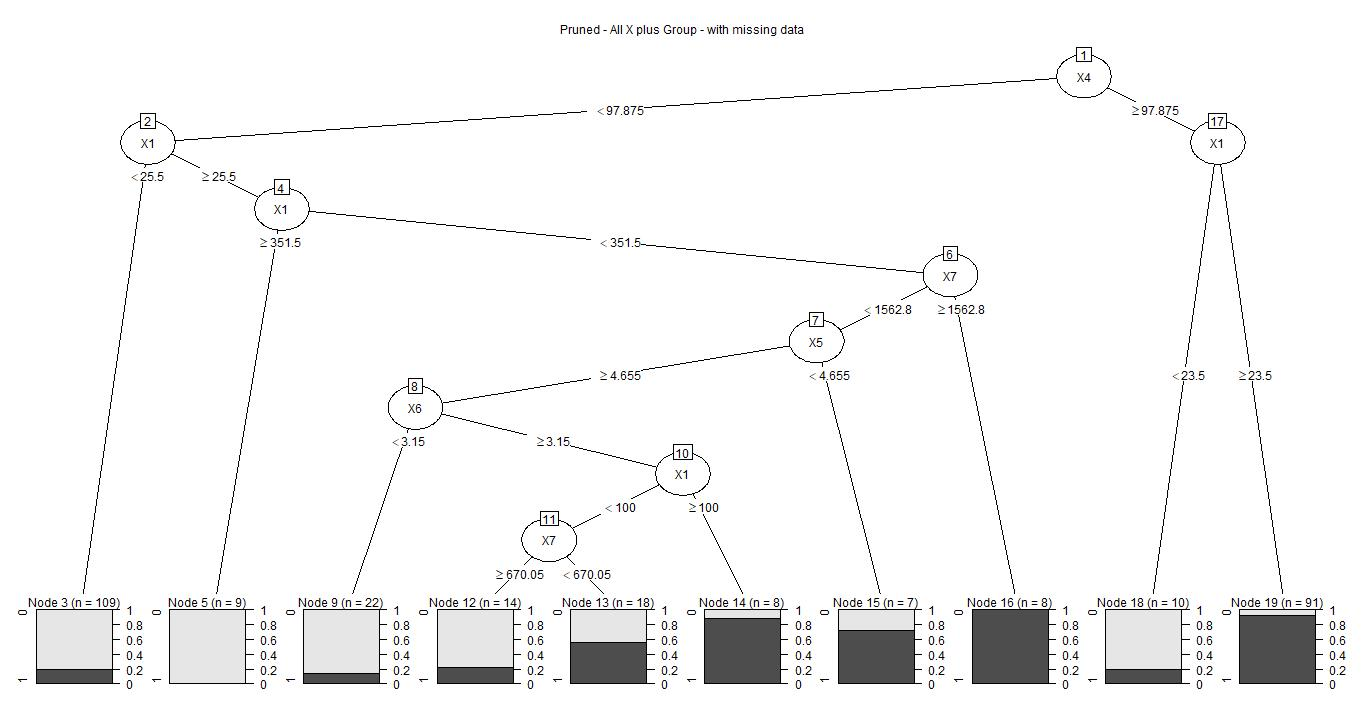
\includegraphics[width=0.7\textwidth, height=8cm]{AllXPlusGroup-withMissingData.jpg}
\textbf{\caption{\label{fig:AllXG}Pruned Decision Tree - All X plus Group variable as predictors before data imputation}}
\end{figure}

\begin{figure}[H]
\centering
\includegraphics[width=0.7\textwidth, height=8cm]{{"All X plus Group - with kNN imputed Data"}.jpg}
\textbf{\caption{\label{fig:AllXGpost}Pruned Decision Tree - All X plus Group variable as predictors after data imputation}}
\end{figure}

\clearpage
    \item \textbf{All Y variables}\\\\
Data imputation had an impact on the decision tree, when built with only Y variables as the predictors. Without imputation, the root node was Y5 and the best number of splits were 4, while after imputation, Y2 was the root node and the best number of splits were 3 as shown in \prettyref{fig:AllY} and \prettyref{fig:AllYpost}.
\begin{figure}[H]
\centering
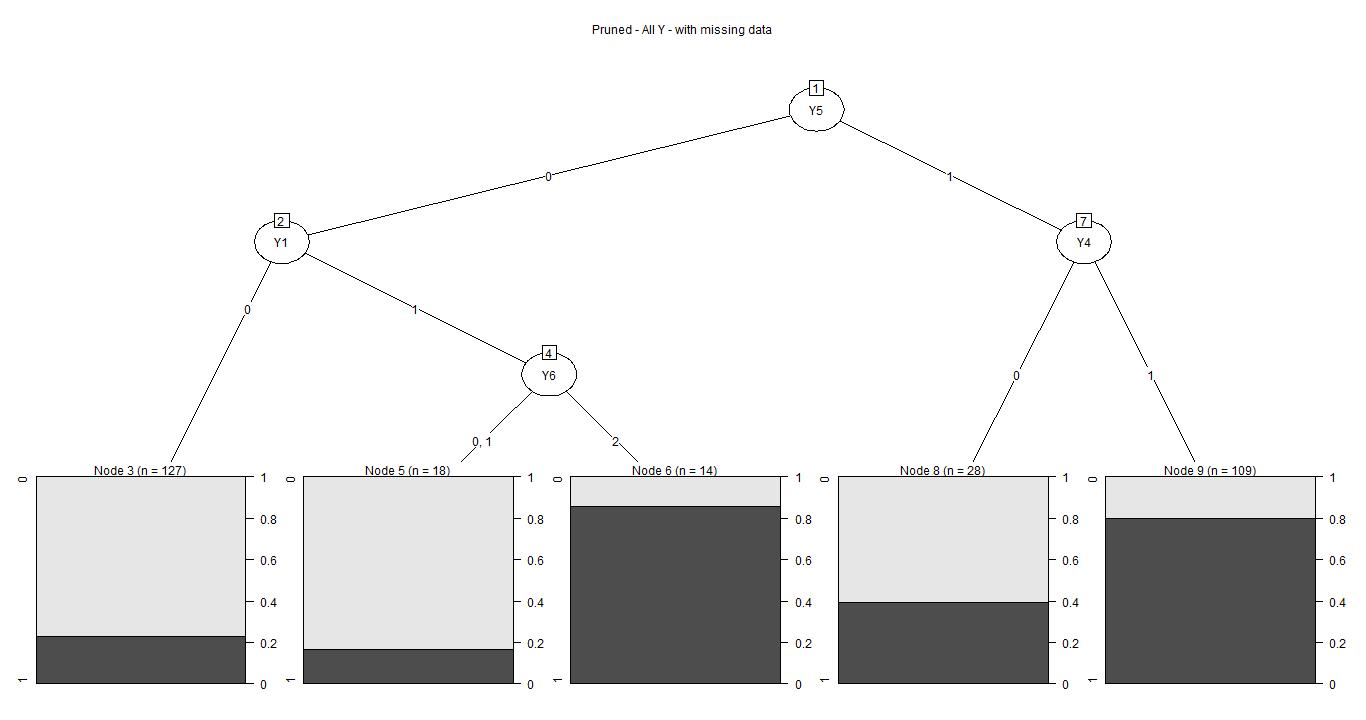
\includegraphics[width=0.7\textwidth, height=8cm]{AllY-withMissingData.jpg}
\textbf{\caption{\label{fig:AllY}Pruned Decision Tree - All Y variables as predictors before data imputation}}
\end{figure}

\begin{figure}[H]
\centering
\includegraphics[width=0.7\textwidth, height=8cm]{{"All Y - with kNN imputed Data"}.jpg}
\textbf{\caption{\label{fig:AllYpost}Pruned Decision Tree - All Y variables as predictors after data imputation}}
\end{figure}

\clearpage
    \item\textbf{All Y variables plus Group}\\\\
Considering "Group" along with the Y variables had some impact on the decision trees. The decision tree without imputation in \prettyref{fig:AllYG} remained similar to the pre-imputation decision tree with only Y variables, with Y5 as the root node and best number of splits were 4, while after imputation, Y2 was the root node and the only split, leading to an underfitted model. Though "Group" wasn't considered for a split, its introduction reduced the number of splits to 1, while using the imputed dataset as shown in \prettyref{fig:AllYGpost}.
\begin{figure}[H]
\centering
\includegraphics[width=\textwidth, height=8cm]{{"All Y plus group - with missing data"}.jpg}
\textbf{\caption{\label{fig:AllYG}Pruned Decision Tree - All Y plus Group variable as predictors before data imputation}}
\end{figure}

\begin{figure}[H]
\centering
\includegraphics[width=\textwidth, height=8cm]{{"All Y plus group - with kNN imputed Data"}.jpg}
\textbf{\caption{\label{fig:AllYGpost}Pruned Decision Tree - All Y plus Group variable as predictors after data imputation}}
\end{figure}
    
\clearpage
        \item\textbf{All variables}\\\\
When all the variables were considered for building a decision tree, pre-imputation, only 2 splits with X4 and X1 were found to be the best as shown in \prettyref{fig:All}. Post-imputation, X4 remained as the primary split, with the total number of splits as 5. Only 1 Y variable, Y1 was used for a split, the remaining 4 were all X variables - X4, X1, X5 and X6 as shown in \prettyref{fig:Allpost}.
\begin{figure}[H]
\centering
\includegraphics[width=\textwidth, height=8cm]{{"All inputs - with missing data"}.jpg}
\textbf{\caption{\label{fig:All}Pruned Decision Tree - All variables as predictors before data imputation}}
\end{figure}

\begin{figure}[H]
\centering
\includegraphics[width=\textwidth, height=8cm]{{"All inputs - with kNN imputed Data"}.jpg}
\textbf{\caption{\label{fig:Allpost}Pruned Decision Tree - All variables as predictors after data imputation}}
\end{figure}

\end{enumerate}

\clearpage
\textcolor{titleBlue}{\subsection{Random Forest}}
\label{sec:randomforest}
Random forest models were created using all the variables in the dataset in both the cases, with and without data imputation.
From the variable importance plots in \prettyref{fig:prevarimp} and \prettyref{fig:postvarimp} it is evident that the X variables are significantly more important to predicting "Response", than the Y variables or the "Group" variable. 
Before and after data imputation, X4 was the most important variable with the lowest impurity. All the X variables were the better predictors in both cases over the Y variables and the "Group" variable.
\begin{figure}[H]
\centering
\includegraphics[width=\textwidth, height=8cm]{{"RF - with missing dataVariable Importance Plot"}.jpg}
\textbf{\caption{\label{fig:prevarimp}Variable Importance Plot before data imputation}}
\end{figure}

\begin{figure}[H]
\centering
\includegraphics[width=\textwidth, height=8cm]{{"RF - with kNN imputed Variable Importance Plot"}.jpg}
\textbf{\caption{\label{fig:postvarimp}Variable Importance Plot after data imputation}}
\end{figure}
\clearpage
The error plots in \prettyref{fig:preerror} and \prettyref{fig:posterror} show decreasing trends in prediction errors with an increase in the number of decision tree classifiers. The green line represents classification error for class "1", black line represents out-of-bag error and the red line represents classification error for class "0". 
The misclassification and out-of-bag error rate is slightly lower when using the imputed dataset.
\begin{figure}[H]
\centering
\includegraphics[width=\textwidth, height=8cm]{{"RF - with missing dataError Plot"}.jpg}
\textbf{\caption{\label{fig:preerror}Error Plot before data imputation}}
\end{figure}

\begin{figure}[H]
\centering
\includegraphics[width=\textwidth, height=8cm]{{"RF - with kNN imputed DataError Plot"}.jpg}
\textbf{\caption{\label{fig:posterror}Error Plot after data imputation}}
\end{figure}
\clearpage
\textcolor{titleBlue}{\section{Conclusion}}
\label{sec:conclusion}
The analysis of the given dataset in this project showed that X4 is the most important predictor of the "Response" label. In general, all the X variables provided a better understanding of the target label than the Y variables or the "Group" variable.
The above conclusion can be attributed to 2 reasons as per the findings of this project:
\begin{enumerate}
    \item The high importance of X4 can be attributed to the fact that X4 was the only variable (consequently Y4 also, since it is derived from X4) that did not have any missing data originally as shown in \prettyref{fig:missingPre}. This meant that X4 had accurate values and hence gave the purest information about the target label
    \item All the X variables were better predictors than the Y variables since Y variables were derived from X. Also, X variables were continuous and provided more specific information than Y variables, which were categorical, and the class of each Y variable was determined by a range of values of the respective X attribute
\end{enumerate}
\end{document}